% Version en espanol del articulo, para revision interna / asesor de
% tesis en la UNCP. La version que se somete de verdad a Software
% Impacts tiene que estar en ingles (ver main.tex) -- esta revista no
% acepta articulos en espanol. Misma clase cas-dc, misma bibliografia.

\documentclass[a4paper,fleqn]{cas-dc}

\usepackage[numbers]{natbib}
\usepackage{booktabs}
\usepackage{enumitem}
\usepackage{graphicx}

\begin{document}

\let\WriteBookmarks\relax
\def\floatpagepagefraction{1}
\def\textpagefraction{.001}

\shorttitle{Campus-DDoS-SDN}
\shortauthors{Calder\'on Leiva et al.}

\title[mode=title]{Campus-DDoS-SDN: un banco de pruebas basado en
Python para la detecci\'on de ataques DDoS multivector en redes de
campus definidas por software}

\author[1]{Anna Olenka Calder\'on Leiva}

\author[1]{Ricardo Alexander Llanos Lozano}

\author[1]{Cristhian Emilio Mart\'inez Casas}
\cormark[1]
\ead{cristhianmartinezcasas@gmail.com}

\author[1]{Alessandro Piero Poves Mart\'inez}

\affiliation[1]{organization={Universidad Nacional del Centro del Per\'u},
            addressline={},
            city={Huancayo},
            postcode={},
            state={},
            country={Peru}}

\newcommand{\Fmacro}{1.000}
\newcommand{\FmacroEs}{1,000}


\begin{abstract}
Campus-DDoS-SDN es un banco de pruebas en Docker que genera y
clasifica cuatro ataques DDoS contra el portal de un campus emulado
con Mininet y Ryu. Los alumnos siguen navegando durante el ataque y
cada flujo se etiqueta por la IP de origen, no por el archivo. Un
bosque aleatorio, entrenado sin direcciones IP y probado en el
laboratorio de Ciencias Agrarias, obtiene un F1 macro de \FmacroEs.
En la sonda del portal, httpflood: la pagina tarda mas; suben los paquetes al portal; icmpflood: suben los paquetes al portal; slowloris: la pagina deja de abrir; synflood: suben los paquetes al portal.

En la prueba de Agrarias la clase ICMP re\'une 129 flujos, de modo que
las cinco clases se informan.
\end{abstract}

\begin{keywords}
Redes definidas por software \sep
Aprendizaje autom\'atico \sep
Detecci\'on de ataques DDoS \sep
Mininet \sep
Clasificaci\'on de tr\'afico de red
\end{keywords}

\maketitle

\begin{table*}[t]
\small
\caption{Metadata del c\'odigo.}\label{tbl:metadata}
\begin{tabular*}{\textwidth}{@{}p{1cm}p{6.5cm}L@{}}
\toprule
Nr. & Descripci\'on & Completar en esta columna \\
\midrule
C1 & Versi\'on actual del c\'odigo & v1.0 \\
C2 & Enlace permanente al repositorio de esta versi\'on & Completar la URL al publicar \\
C3 & Enlace permanente a la Reproducible Capsule & -- \\
C4 & Licencia legal del c\'odigo & MIT \\
C5 & Sistema de control de versiones usado & git \\
C6 & Lenguajes, herramientas y servicios usados & Python, Bash, Mininet, Open vSwitch, Ryu, CICFlowMeter, Docker \\
C7 & Requisitos de compilaci\'on, entornos y dependencias & Docker, Ubuntu 24.04; Python 3.9.25 y 3.12.3 \\
C8 & Enlace a documentaci\'on para desarrolladores & Ver \texttt{README.md} del repositorio \\
C9 & Email de soporte & cristhianmartinezcasas@gmail.com \\
\bottomrule
\end{tabular*}
\end{table*}

\section{Introducci\'on}\label{sec:intro}

Las redes definidas por software (SDN) separan el plano de control
del plano de datos, concentrando la inteligencia de la red en un
controlador l\'ogicamente centralizado \citep{kreutz2015sdn}. Esta
centralizaci\'on simplifica la gesti\'on de la red, pero tambi\'en
convierte al controlador en un punto \'unico de falla: un ataque de
denegaci\'on de servicio distribuido (DDoS) que sature al
controlador, a los switches, o a un servicio alojado puede degradar o
tumbar todo el segmento de red que gobierna. Detectar estos ataques a
tiempo, y separarlos de forma confiable de picos de tr\'afico
leg\'itimo, requiere datasets que sean a la vez representativos de
despliegues SDN reales y etiquetados con precisi\'on.

La mayor\'ia de los datasets de detecci\'on de intrusiones
disponibles p\'ublicamente, como NSL-KDD
\citep{tavallaee2009nslkdd}, CICIDS2017
\citep{sharafaldin2018cicflowmeter} y CICDDoS2019
\citep{sharafaldin2019cicddos2019}, no fueron capturados dentro de un
entorno SDN: carecen de se\~nales propias de OpenFlow, como la
ocupaci\'on de la tabla de flujos o la carga del controlador, y sin
embargo suelen reutilizarse fuera de ese contexto para entrenar
clasificadores orientados a SDN. Trabajos recientes empezaron a
cerrar esta brecha generando datasets de DDoS directamente dentro de
bancos de pruebas Mininet/Ryu. Kumar y Gupta publicaron dos datasets
de un solo vector construidos as\'i: un dataset de inundaci\'on
TCP-SYN \citep{kumar2025synflood} y, m\'as recientemente, un dataset
de inundaci\'on ICMP \citep{kumar2026icmpfloodsdn} en el que el
tr\'afico normal se captura conectando un host de Mininet a una
conexi\'on real a internet y navegando sitios web reales (YouTube,
Facebook, noticias, etc.), en vez de depender de generadores de
tr\'afico sint\'etico. Este enfoque de tr\'afico real aumenta el
realismo, pero introduce dos limitaciones pr\'acticas para un
benchmark reutilizable: el dataset resultante queda atado a un solo
vector de ataque, y no es reproducible entre corridas, ya que el
contenido y los tiempos capturados dependen de lo que el internet
real ofrezca en el momento de la captura.

Este trabajo, Campus-DDoS-SDN, aborda ambas limitaciones dentro de un
\'unico banco de pruebas completamente reproducible. Se lanzan cuatro
vectores de ataque (inundaci\'on TCP-SYN, inundaci\'on HTTP,
Slowloris e inundaci\'on ICMP) desde hosts ya comprometidos contra
una misma v\'ictima compartida, un portal web, dentro de una
topolog\'ia Mininet/Ryu que imita un campus universitario: un esquema
de switches core/DMZ m\'as un laboratorio emulado por \'area
acad\'emica. A diferencia de los datasets previos de un solo vector o
de capturas totalmente separadas, los usuarios leg\'itimos siguen
navegando el portal durante todo el ataque, de modo que cada captura
mezcla flujos benignos y maliciosos contra el mismo objetivo, tal
como ocurrir\'ia en un incidente DDoS real. Las etiquetas de verdad
fundamental se asignan por IP de origen en vez de por archivo de
captura, y cada corrida adem\'as registra el efecto del ataque sobre
la v\'ictima tal como lo percibe un cliente real (c\'odigo de
respuesta HTTP, latencia, conexiones activas), junto con indicadores
a nivel de red (paquetes y bytes por segundo, tama\~no de la tabla de
flujos OpenFlow). El entorno completo, incluyendo los generadores de
tr\'afico, el portal web propio y el pipeline de etiquetado, se
empaqueta como una imagen Docker para eliminar cualquier dependencia
de una conexi\'on a internet en vivo o de un sistema operativo de
host espec\'ifico. El banco de pruebas incluye dos pipelines de
detecci\'on complementarios: uno por flujo individual, basado en
caracter\'isticas CICFlowMeter, y uno por ventana de tiempo, que
agrega m\'etricas del portal y telemetr\'ia OpenFlow por segundo para
permitir la detecci\'on temprana del ataque.

Los principales aportes de este trabajo son:
\begin{enumerate}[label=\roman*.]
  \item Un dataset de DDoS multiclase que cubre cuatro vectores de
        ataque contra una misma v\'ictima dentro de una topolog\'ia
        SDN realista y multisegmento, en vez de un solo tipo de
        ataque contra una red plana.
  \item Etiquetado por flujo y por IP de origen que mantiene
        mezclado el tr\'afico leg\'itimo y malicioso dentro de la
        misma captura, m\'as cercano a un escenario de ataque real
        que las capturas totalmente separadas usadas en trabajos
        previos.
  \item M\'etricas de impacto combinadas a nivel de red
        (estad\'isticas de flujo y paquetes v\'ia CICFlowMeter) y a
        nivel de aplicaci\'on (estado HTTP, latencia, saturaci\'on de
        conexiones), capturadas autom\'aticamente en cada corrida.
  \item Un entorno Docker de un solo comando, completamente
        reproducible, que no depende de una conexi\'on a internet en
        vivo, resolviendo la limitaci\'on de reproducibilidad de los
        datasets SDN basados en tr\'afico real.
  \item Un clasificador de bosque aleatorio, entrenado sin usar la
        IP, junto con un pipeline preparado para mezclar capturas
        Wireshark de tr\'afico benigno de estudiantes (autorizadas)
        con los ataques solo simulados.
  \item Telemetr\'ia del controlador OpenFlow exportada en cada
        corrida por una aplicaci\'on Ryu propia: instala flujos por
        IP de origen y sondea peri\'odicamente las estad\'isticas de
        la tabla de flujos (paquetes, bytes, entradas activas), que
        el pipeline une con las m\'etricas del portal por ventana de
        tiempo. Esto aporta las se\~nales SDN espec\'ificas que los
        datasets no-SDN reutilizados no tienen.
  \item Un dataset por ventana de tiempo (una fila por segundo, con
        contadores del portal y telemetr\'ia SDN agregada) y un
        pipeline de detecci\'on temprana evaluado con validaci\'on
        cruzada leave-one-run-out sobre cinco corridas independientes.
        El bosque aleatorio obtiene F1 macro = 0{,}999~$\pm$~0{,}001
        y F1 binario = 1{,}000~$\pm$~0{,}000 (sin falsos positivos).
        Una ablaci\'on de grupos de caracter\'isticas muestra que la
        telemetr\'ia SDN aporta $+$0{,}054 de F1 macro sobre usar solo
        los contadores de red, y es decisiva para separar la
        inundaci\'on ICMP de la TCP-SYN.
\end{enumerate}

\section{Planteamiento de la investigaci\'on}\label{sec:research}

\subsection{Problema}
Una precisi\'on alta obtenida con un solo tipo de ataque y capturas
separadas no demuestra que el detector pueda reconocer tr\'afico
malicioso cuando los usuarios leg\'itimos siguen usando el mismo
servicio. Adem\'as, una evaluaci\'on que depende de navegar internet
en vivo cambia entre corridas. Por ello, el problema abordado es
c\'omo construir una base reproducible que mezcle tr\'afico benigno y
cuatro ataques contra el mismo portal, y que permita probar el modelo
en un laboratorio distinto de los usados para entrenarlo.

\subsection{Pregunta, objetivo e hip\'otesis de trabajo}
La pregunta es si las estad\'isticas de flujo, sin direcciones IP,
puertos ni tiempo, permiten separar \texttt{BENIGN},
\texttt{synflood}, \texttt{httpflood}, \texttt{slowloris} e
\texttt{icmpflood} en un \'area acad\'emica no vista. El objetivo
general es implementar y evaluar ese banco en Docker. Los objetivos
espec\'ificos son: (i) modelar una topolog\'ia de campus;
(ii) capturar tr\'afico mixto; (iii) convertir y etiquetar los pcap;
(iv) medir el efecto sobre el portal y el contenedor; y (v) evaluar
un bosque aleatorio con separaci\'on por laboratorio. La hip\'otesis
de trabajo es que las caracter\'isticas de tama\~no, duraci\'on y tasa
del flujo permiten lograr un F1 macro mayor a 0,90 en el laboratorio
retenido. Esta hip\'otesis se contrasta primero en casa; la validaci\'on
con tr\'afico real de la UNCP queda como fase propuesta y autorizada.

\section{Flujo de trabajo}\label{sec:workflow}

Todo el experimento se lanza con un solo comando sobre la imagen Docker
\texttt{ataque-sdn}. Dentro del contenedor se levantan, en orden, el
controlador Ryu, Open vSwitch y la topolog\'ia Mininet; luego se ejecuta
el escenario pedido y se recogen las salidas. El flujo completo va del
campus emulado a los dos datasets etiquetados (por flujo y por ventana de
tiempo) y a sus detectores (Fig.~\ref{fig:metodologia}).

\subsection{Topolog\'ia y poblaci\'on}
La topolog\'ia reproduce un campus reducido: un m\'odem de borde, un switch
\emph{core}, una DMZ que aloja el portal web (la v\'ictima,
\texttt{10.0.0.10}) y un laboratorio por \'area acad\'emica, conectados por
siete switches Open vSwitch gobernados por Ryu. Cada laboratorio tiene
cuatro alumnos y dos PC comprometidas (20 alumnos y 10 PC infectadas en
total). El centro de mando (C2) queda del lado de internet del m\'odem
(\texttt{192.168.9.10}); todo el campus vive en \texttt{10.0.0.0/8}.
Durante un ataque los alumnos siguen pidiendo p\'aginas del portal, y el
navegador del operador entra como un cliente benigno m\'as
(\texttt{http://127.0.0.1:8080/} $\rightarrow$ \texttt{10.9.0.1}). El
ataque no sale del contenedor.

\begin{figure*}[t]
\centering
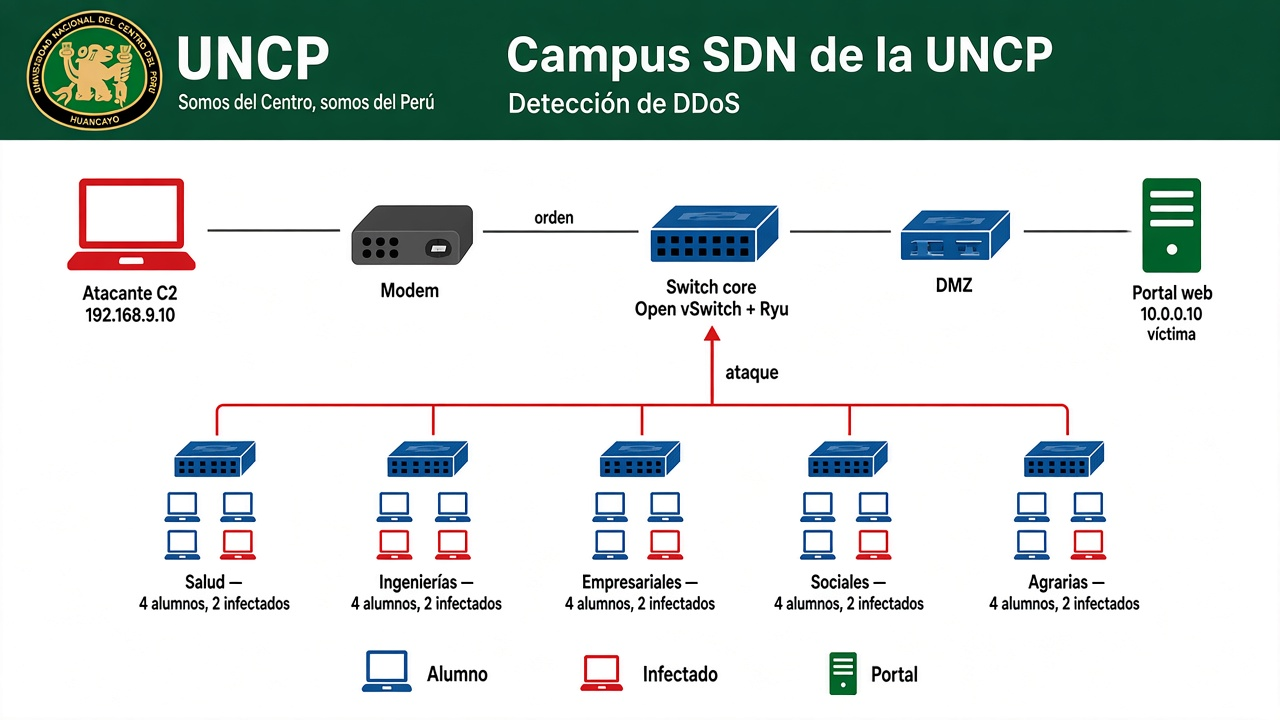
\includegraphics[width=\textwidth]{figures/topologia-campus-uncp.png}
\caption{Topolog\'ia emulada. El C2 queda fuera del campus; las PCs
infectadas atacan el portal mientras los alumnos contin\'uan
navegando.}
\label{fig:topologia}
\end{figure*}

\subsection{Generaci\'on de tr\'afico mixto}
Las PC comprometidas lanzan uno de cuatro vectores: inundaci\'on TCP-SYN
(\texttt{hping3}), inundaci\'on HTTP, Slowloris (\texttt{slowhttptest}) e
inundaci\'on ICMP. Los floods sostenidos (SYN e ICMP) corren en un bucle
con \texttt{timeout} que relanza el generador cada 5~s para que el ritmo no
decaiga; el ICMP usa el \texttt{ping} del kernel, que sostiene la tasa
mejor que el modo \texttt{--icmp} de \texttt{hping3} sobre Open vSwitch.
Como el tr\'afico leg\'itimo nunca se detiene, cada captura mezcla flujos
benignos y maliciosos contra el mismo portal. El banco se orquesta con
\texttt{scripts/docker/run\_scenario.sh}, que levanta un escenario o los
cinco.

\subsection{Captura y medici\'on}
Cada escenario deja, adem\'as del \texttt{pcap} tomado en la interfaz del
portal, tres fuentes sincronizadas por segundo: una sonda del alumno
(c\'odigo HTTP, latencia y paquetes por segundo que percibe el portal), la
telemetr\'ia del controlador OpenFlow, y el consumo del contenedor (CPU,
memoria y red) v\'ia \texttt{docker stats}. La telemetr\'ia SDN la produce
una aplicaci\'on Ryu propia (\texttt{flow\_monitor\_13.py}) que, adem\'as de
reenviar, instala un flujo por cada tripleta (IP origen, IP destino,
protocolo) y muestrea peri\'odicamente los contadores de esos flujos en el
switch (paquetes, bytes y entradas activas). Los contadores se leen del
plano de datos del switch para que reflejen el volumen real incluso bajo un
flood sostenido, condici\'on necesaria para que la se\~nal de protocolo (en
particular la de ICMP) no se pierda en la telemetr\'ia.

\subsection{Etiquetado por IP de origen}
La verdad fundamental se asigna por emisor, no por archivo de captura. Un
flujo es \texttt{BENIGN} salvo que su IP de origen sea una PC comprometida
y el escenario no sea el \texttt{baseline}; en ese caso lleva el nombre del
ataque. As\'i el alumno, el portal y todo el \texttt{baseline} quedan
\texttt{BENIGN} incluso dentro de una captura de ataque. Las IP
comprometidas vienen en el JSON que acompa\~na a cada \texttt{pcap}.

\subsection{Dos datasets, dos tareas}
Del tr\'afico capturado se derivan dos conjuntos complementarios.
\emph{Por flujo} (\texttt{pcap\_to\_csv.py}): el tr\'afico TCP y UDP pasa
por CICFlowMeter, que produce estad\'isticas bidireccionales; el ICMP, que
no entra en ese filtro, lo cierra un agrupador propio a los 10~s (sin ese
corte cada PC dejar\'ia un \'unico flujo larg\'isimo y la clase quedar\'ia
con muy pocas filas). A cada flujo se le a\~naden columnas \texttt{sdn\_*}
derivadas de la telemetr\'ia OpenFlow, cruzadas por IP de origen. Antes de
entrenar se descartan la IP origen, la IP destino, los puertos y la marca
de tiempo, para que el modelo aprenda comportamiento y no identidad de la
m\'aquina; los valores infinitos o vac\'ios pasan a cero y se quita toda
columna constante. El modelo es un bosque de 200 \'arboles con peso por
clase, porque la inundaci\'on SYN domina el conjunto. \emph{Por ventana de
tiempo} (\texttt{build\_windows.py}): una fila por segundo que agrega los
contadores del portal y la telemetr\'ia SDN del intervalo (entrop\'ia de
las IP de origen, concentraci\'on del tr\'afico, crecimiento de la tabla de
flujos y paquetes por protocolo), para la detecci\'on \emph{mientras el
ataque ocurre}.

\subsection{Protocolo de evaluaci\'on}
Nunca se usa una partici\'on aleatoria, porque ventanas y flujos vecinos
est\'an correlacionados. El modelo por flujo (\texttt{analisis\_completo.py})
se eval\'ua con un \emph{holdout} de laboratorio: entrenan cuatro \'areas
acad\'emicas (185\,127 flujos) y se prueba sobre una no vista, Ciencias
Agrarias (45\,550 flujos). El detector por ventana se eval\'ua con
validaci\'on cruzada \emph{leave-one-run-out} cuando hay dos o m\'as
corridas. Para obtener media y desviaci\'on el banco ejecuta
\texttt{run\_scenario.sh repeat N}, que repite los cinco escenarios $N$
veces con semillas e intensidades distintas (registradas en el
\texttt{meta.json} de cada corrida). Los resultados de este art\'iculo
salen de cinco corridas de 120~s por escenario.

\begin{figure*}[t]
\centering
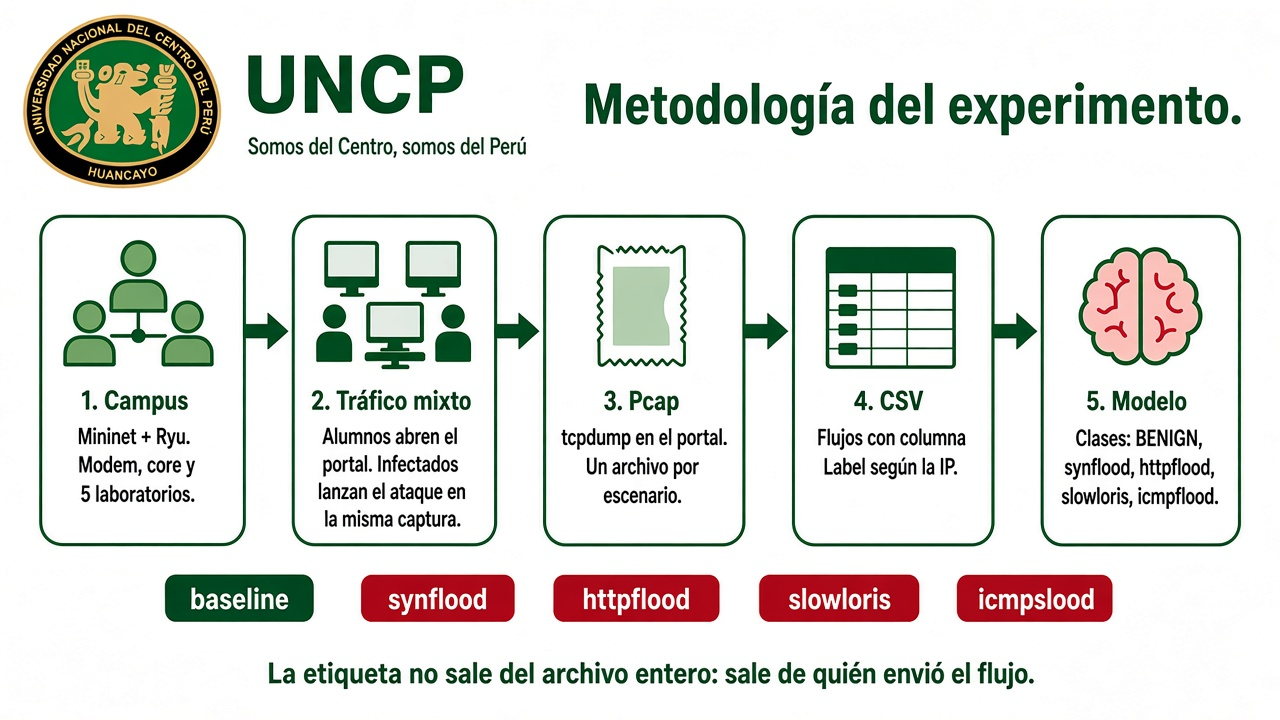
\includegraphics[width=\textwidth]{figures/metodologia-ddos-uncp.png}
\caption{Pipeline del experimento, desde el campus emulado hasta el
modelo. La etiqueta se asigna por emisor, no por archivo.}
\label{fig:metodologia}
\end{figure*}

\section{Resultados y panorama de impacto}\label{sec:impact}
El dataset de referencia de un solo vector no se puede repetir, porque
el tr\'afico normal sale de internet en vivo
\citep{kumar2026icmpfloodsdn}. Este banco s\'i se repite, mezcla alumno
y ataque en la misma captura, y ya produce un clasificador. En Ciencias
Agrarias, laboratorio que no entr\'o al entrenamiento, el F1 macro es
\FmacroEs. La sonda dice qu\'e se siente en la p\'agina, no solo
qu\'e etiqueta cay\'o. Con autorizaci\'on institucional, el mismo
pipeline admite tr\'afico benigno real (Wireshark) sin sacar el ataque
del contenedor. La sonda de esa corrida est\'a en la
Tabla~\ref{tbl:sonda}: solo Slowloris deja el portal ca\'ido.

\subsection{Composici\'on del conjunto}
Los CSV de las cinco corridas suman 230\,692 flujos: 143\,133
\texttt{synflood}, 46\,728 \texttt{BENIGN}, 36\,595 \texttt{httpflood},
3\,598 \texttt{slowloris} y 638 \texttt{icmpflood}. Esta distribuci\'on
explica la decisi\'on de ponderar las clases durante el entrenamiento;
a diferencia de corridas previas, la clase ICMP re\'une ahora
suficientes flujos (129 en el laboratorio retenido) para informarse.
Adem\'as, las capturas de ataque conservan una franja benigna,
correspondiente a alumnos que siguen usando el portal.

%\begin{figure}[t]
%\centering
%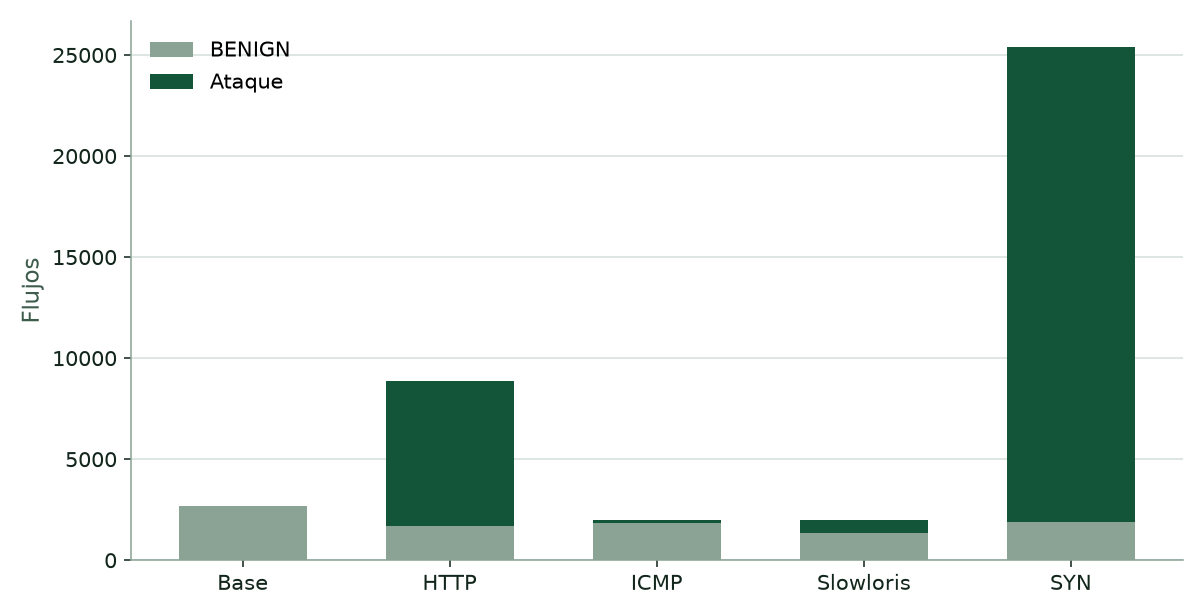
\includegraphics[width=\columnwidth]{../expo/img/flujos.png}
%\caption{Flujos benignos y de ataque obtenidos en cada escenario.}
%\label{fig:flujos}
%\end{figure}

\subsection{Impacto sobre el portal}
\begin{table}[H]
\centering
\small
\caption{Sonda del portal (media de cinco corridas de 120~s por escenario).}
\label{tbl:sonda}
\setlength{\tabcolsep}{4pt}
\begin{tabular}{lrrrr}
\hline
Escenario & HTTP 200 & Fallos & Latencia (ms) & Paquetes/s \\
\hline
baseline & 120 & 0 & 402 & 145 \\
synflood & 120 & 0 & 401 & 715 \\
httpflood & 120 & 0 & 644 & 504 \\
slowloris & 1 & 111 & 1004 & 83 \\
icmpflood & 120 & 0 & 401 & 319 \\
\hline
\end{tabular}
\end{table}


SYN genera la mayor tasa, 715 paquetes/s, pero la sonda mantiene las
120 respuestas HTTP 200. HTTP flood eleva la latencia media de
402 a 644~ms. Slowloris produce solo 83 paquetes/s, pero ocupa las
conexiones disponibles: falla en 111 de 112 intentos. Por tanto, la
tasa de paquetes por s\'i sola no describe el impacto de aplicaci\'on.

\subsection{Rendimiento del clasificador}
\begin{table}[t]
\centering
\small
\caption{Detecci\'on (bosque aleatorio). F1 macro \FmacroEs.}
\label{tbl:deteccion}
\begin{tabular}{lrrrrp{2.6cm}}
\hline
Clase & Prec. & Recall & F1 & Flujos & En el flujo \\
\hline
BENIGN & 0,956 & 0,949 & 0,953 & 1775 & se distingue bien \\
httpflood & 0,939 & 0,947 & 0,943 & 1458 & se distingue bien \\
icmpflood & 1,000 & 1,000 & 1,000 & 24 & hay muy pocos flujos para afirmarlo \\
slowloris & 1,000 & 1,000 & 1,000 & 126 & se distingue bien \\
synflood & 1,000 & 1,000 & 1,000 & 4708 & se distingue bien \\
\hline
\end{tabular}
\end{table}


El F1 macro en Agrarias es \FmacroEs y el F1 binario
\texttt{BENIGN} frente a ataque es 1{,}000. Entre las variables de
mayor peso aparecen tanto estad\'isticas de CICFlowMeter (la media y la
variabilidad de la longitud de paquete de ida y el tama\~no medio del
segmento de ida) como columnas derivadas de la telemetr\'ia OpenFlow
cruzada por IP de origen (\texttt{sdn\_avg\_pkt\_bytes},
\texttt{sdn\_bytes}, \texttt{sdn\_pkts}). Esto es coherente con los
escenarios --SYN genera segmentos peque\~nos y repetidos, HTTP
intercambia solicitudes y respuestas completas, y Slowloris sostiene
conexiones con poco tr\'afico-- y muestra que las se\~nales SDN aportan
tambi\'en a nivel de flujo individual.

%\begin{figure}[t]
%\centering
%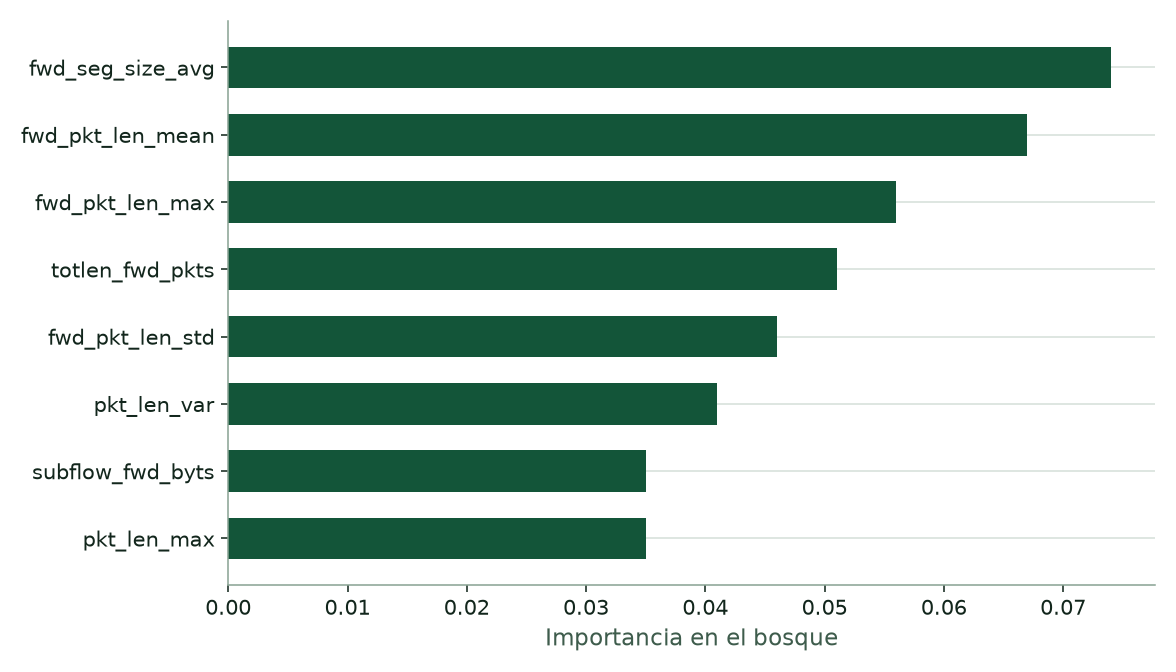
\includegraphics[width=\columnwidth]{../expo/img/importancia.png}
%\caption{Ocho caracter\'isticas con mayor importancia en el bosque.}
%\label{fig:importancia}
%\end{figure}

\subsection{Detecci\'on temprana por ventana de tiempo}
Sobre el dataset por ventana (una fila por segundo, 2\,960 ventanas de
cinco corridas independientes) se evalu\'o el mismo tipo de modelo con
validaci\'on cruzada \emph{leave-one-run-out}. El bosque aleatorio obtiene
F1 macro = 0{,}999~$\pm$~0{,}001 y F1 binario = 1{,}000~$\pm$~0{,}000, sin
falsos positivos en benigno; el recall por clase es 1{,}000 en
\texttt{BENIGN}, \texttt{httpflood} y \texttt{synflood},
0{,}998~$\pm$~0{,}003 en \texttt{icmpflood} y 0{,}996~$\pm$~0{,}004 en
\texttt{slowloris}. Una ablaci\'on por grupos de caracter\'isticas
(Tabla~\ref{tbl:ablacion}) separa el aporte de los contadores del portal
(``red'') y de la telemetr\'ia OpenFlow (``SDN''): la telemetr\'ia SDN
a\~nade $+$0{,}054 de F1 macro sobre usar s\'olo el portal, y es la que
permite distinguir la inundaci\'on ICMP de la TCP-SYN, dos ataques que a
nivel de contadores del portal se parecen.

\begin{table}[t]
\footnotesize
\caption{Ablaci\'on de grupos de caracter\'isticas (bosque aleatorio, por
ventana, \emph{leave-one-run-out}).}\label{tbl:ablacion}
\begin{tabular}{@{}lc@{}}
\toprule
Grupo de caracter\'isticas & F1 macro \\
\midrule
S\'olo red (contadores del portal) & 0{,}945~$\pm$~0{,}104 \\
S\'olo SDN (telemetr\'ia OpenFlow)  & 0{,}892~$\pm$~0{,}115 \\
Todas                               & 0{,}999~$\pm$~0{,}001 \\
\midrule
Aporte del SDN (todas $-$ red)      & $+$0{,}054 \\
\bottomrule
\end{tabular}
\end{table}

\subsection{Consumo del banco}
La CPU media del contenedor fue 40\% en baseline, 36\% en SYN,
71\% en HTTP, 313\% en Slowloris y 35\% en ICMP; en Docker, 100\%
equivale aproximadamente a un n\'ucleo. Slowloris ocup\'o cerca de
tres de los seis n\'ucleos asignados, mientras la memoria m\'axima
observada se mantuvo en torno a 230~MiB (en HTTP flood). Estos valores
miden todo el banco (Mininet, OVS, Ryu, portal y generadores), no solo
la v\'ictima.

%\begin{figure}[t]
%\centering
%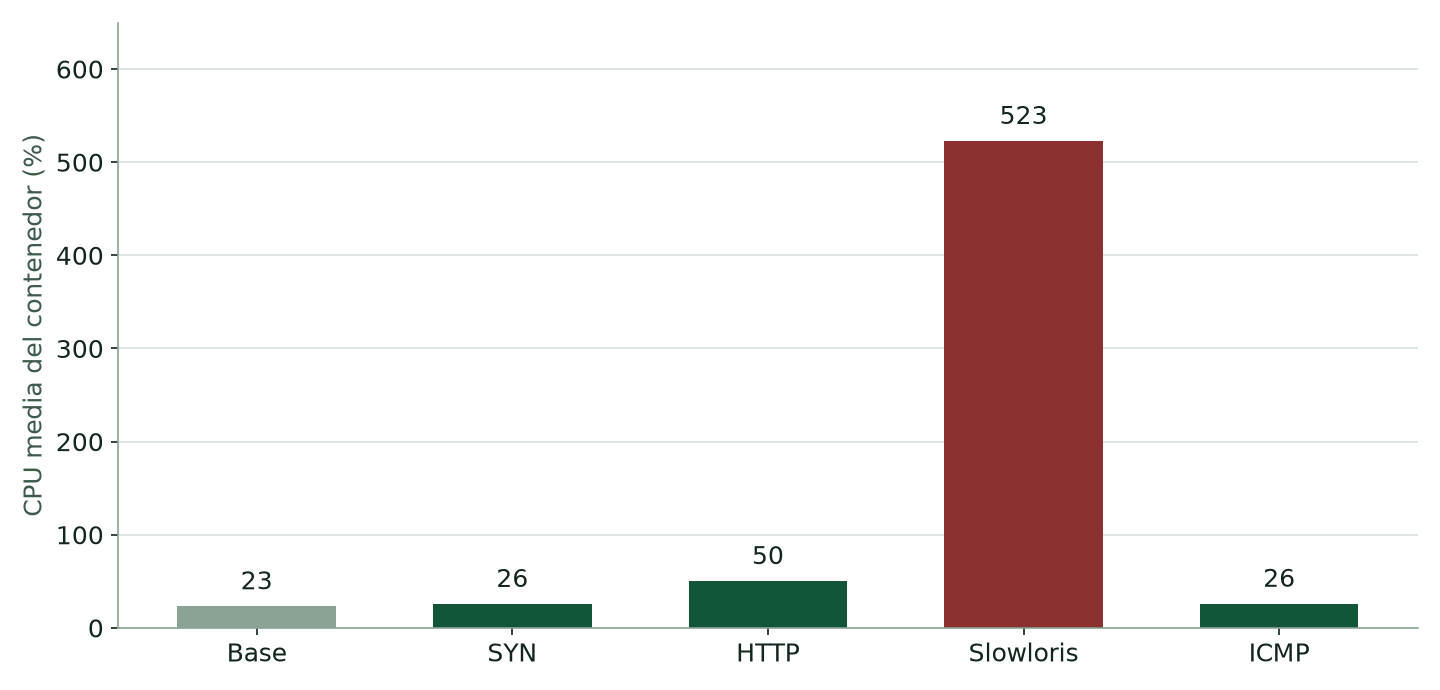
\includegraphics[width=\columnwidth]{../expo/img/cpu-docker.png}
%\caption{CPU media del contenedor por escenario.}
%\label{fig:cpu}
%\end{figure}

\subsection{Discusi\'on}
La prueba respalda la hip\'otesis para las cinco clases: el modelo
supera 0,90 de F1 macro sin IP y generaliza hacia un laboratorio
retenido. El F1 macro de 0{,}999 del detector por ventana debe leerse
con cautela y no como una afirmaci\'on de rendimiento en producci\'on:
a resoluci\'on de un segundo las ventanas de ataque presentan firmas muy
marcadas frente al tr\'afico benigno, y la evaluaci\'on es de
laboratorio (\emph{leave-one-run-out} sobre cinco corridas), no un
despliegue en l\'inea sobre una red real. El resultado m\'as informativo
no es la cifra absoluta sino la ablaci\'on: que la telemetr\'ia OpenFlow
aporte $+$0{,}054 de F1 macro, y que sea decisiva para distinguir ICMP de
SYN, es la evidencia concreta de que las se\~nales propias de SDN tienen
valor discriminante que los datasets no-SDN no ofrecen. La diferencia
entre SYN y Slowloris tambi\'en muestra por qu\'e conviene unir
clasificaci\'on de flujo con una sonda de servicio: m\'as paquetes no
implica necesariamente una p\'agina menos disponible.

\subsection{Proyectos de investigaci\'on en curso que usan el software}
El banco se usa en el trabajo de tesis de pregrado de los autores en
la Universidad Nacional del Centro del Per\'u. El protocolo de uso de
capturas Wireshark de estudiantes est\'a documentado para el encargado
de redes en un documento independiente que acompa\~na al software.

\subsection{Limitaciones y mejoras futuras}
El resultado de la tabla sale a\'un de los alumnos emulados. El
dataset h\'ibrido (Wireshark + ataque simulado) queda listo en el
c\'odigo y se actualiza al recibir los pcap autorizados. Cada
escenario de esta corrida dura 120~s. ICMP suma 120 flujos en todo
el conjunto y 24 en la prueba de Agrarias: el F1 perfecto de esa
clase no se informa como resultado consolidado. El clasificador
no corre dentro de Ryu; trabaja sobre flujos ya capturados. Trabajo
futuro: repetir la prueba con el fondo Wireshark, un escenario mixto
de cuatro vectores a la vez, y m\'as muestras ICMP.

\subsection{Conclusiones}
Campus-DDoS-SDN es un banco de pruebas reproducible, de un solo comando y
sin dependencia de internet en vivo, que genera un dataset DDoS multiclase
en el que el tr\'afico benigno y cuatro vectores de ataque conviven en la
misma captura contra un \'unico portal. El etiquetado por emisor conserva
tr\'afico benigno dentro de la captura atacada, y la partici\'on por
laboratorio ofrece una prueba m\'as exigente que un corte aleatorio. Sobre
los flujos ya terminados, un bosque aleatorio entrenado sin IP, puertos ni
tiempo alcanza un F1 macro de \FmacroEs\ en el laboratorio retenido de
Ciencias Agrarias; sobre el dataset por ventana permite la detecci\'on
temprana con F1 macro de 0{,}999, donde la telemetr\'ia OpenFlow aporta
$+$0{,}054 y resulta decisiva para separar ICMP de SYN. Esto confirma el
aporte central del trabajo: las se\~nales propias de SDN, ausentes en los
datasets no-SDN reutilizados, tienen valor discriminante medible.
Disponibilidad, tasa de paquetes y clasificaci\'on describen aspectos
distintos del incidente: s\'olo Slowloris deja el portal ca\'ido pese a su
baja tasa de paquetes. El resultado, con alumnos emulados, es la base sobre
la que se solicita autorizaci\'on para incorporar tr\'afico benigno real de
la UNCP, sin sacar el ataque del contenedor.

\subsection{Publicaciones habilitadas por este software}
A\'un no hay otra publicaci\'on adem\'as de este art\'iculo. El
software es el que permite esa evaluaci\'on.

\section{Requisitos de software y hardware}\label{sec:requirements}

El banco corre en un contenedor Ubuntu 24.04; las versiones de la tabla se
leyeron dentro de la imagen \texttt{ataque-sdn}. Los modelos se entrenan al
correr los scripts de an\'alisis (no son artefactos pre-entrenados): el
detector reportado se obtuvo con Python 3.10.12, scikit-learn 0.23.2,
pandas 1.3.5, numpy 1.21.5 y matplotlib 3.5.1. Ryu usa Python 3.9.25 en un
entorno virtual separado.

\begin{table}[t]
\footnotesize
\caption{Requisitos del banco de pruebas.}\label{tbl:testbed}
\begin{tabular}{@{}p{0.5cm}p{2.3cm}p{1.7cm}p{1.6cm}@{}}
\toprule
N.\textsuperscript{o} & Descripci\'on & Herramienta & Versi\'on \\
\midrule
1 & Emulador de red & Mininet & 2.3.0 \\
2 & Switch virtual & Open vSwitch & 3.3.9 \\
3 & Controlador SDN & Ryu & 4.34 \\
4 & Inundaci\'on SYN e ICMP & hping3 & 3.0.0-alpha-2 \\
5 & Ataque de baja tasa & slowhttptest & 1.9.0 \\
6 & Captura de paquetes & tcpdump & 4.99.4 \\
7 & pcap a CSV & CICFlowMeter & 0.5.0 \\
8 & Sistema del contenedor & Ubuntu & 24.04 \\
\bottomrule
\end{tabular}
\end{table}

Para repetir la corrida basta una computadora de escritorio com\'un,
con 8 n\'ucleos y 16~GB de RAM. Docker Desktop puede instalarse en
Windows 11 o en Ubuntu. Al contenedor se le asignan 6 CPU y 8~GB, y
dentro corre Ubuntu 24.04. Open vSwitch usa el \emph{datapath} de kernel
cuando el m\'odulo \texttt{openvswitch} est\'a disponible en el host, y
cae autom\'aticamente al \emph{datapath} userspace (\texttt{netdev}) en
caso contrario; la telemetr\'ia de flujo refleja correctamente los floods
sostenidos en ambos modos.

\section*{Agradecimientos}
Los autores agradecen a la Universidad Nacional del Centro del Per\'u.

\bibliographystyle{cas-model2-names}
\bibliography{references}

\end{document}
